\section{Proving}
\label{tut_proving}
\index{proving}

\tick{\textbf{Goals:} The goal of this section is to get familiar with the Proving Perspective and to carry out a simple proof by hand.}

\subsection{The Celebrity Problem}
\label{tut_celebrity_problem}

In this section, we will work on the model of the so-called celebrity problem. In the setting for this problem, we have a ``knows'' relation. This relation is defined so that

\begin{itemize}
	\item no one knows himself,
	\item the celebrity knows nobody,
	\item but everybody knows the celebrity.
\end{itemize}    

The goal is to find the celebrity.

\warning{Make sure that you have no existing Project named Celebrity. If you do, then rename it. To do so, right click the project and select \textsf{Rename...}}

\index{import project}
Import the archive file \file{Celebrity.zip}{Celebrity.zip} to you Event-B Explorer. To do this, select \textsf{File $\rangle $ Import $\rangle $ General $\rangle $ Existing Projects into Workspace}. Then select the according archive file and click on \textsf{Finish}.

Rodin takes a few seconds to extract and load all the files. Once it is done, it shows that there are a few problems with this project as you can see in the Rodin Problems View (compare with figure \ref{fig_tut_08_rodin_problemview}).

\begin{figure}[!ht]
\begin{center}
	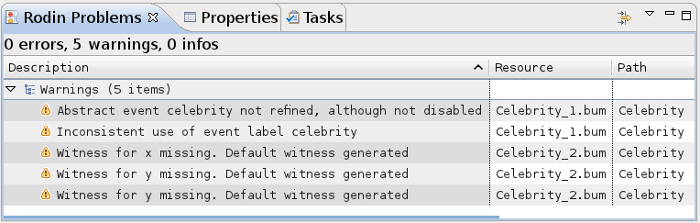
\includegraphics{img/tutorial/tut_08_rodin_problems.png}
	\caption{Warnings in the Rodin Problems View}
	\label{fig_tut_08_rodin_problemview}
\end{center}
\end{figure}

In the first part of this section, our goal is to fix these problems. Let's take a look at the warning stating that the event label ``celebrity'' is misused (``Inconsistent use of event label celebrity''). Double-click on the warning to open the \texttt{Celebrity\_1} machine. Select the event \textsf{celebrity}. The problem is that the event is not declared as a refinement. To solve the problem, expand the event and add a new entry in the \textsf{REFINES} section (Click on the \icon{rodin/add.png} button to create a new entry). This declares that the event is a refinement of an event with the same name in the abstract machine (\ref{abstract_machine}). As this is the case here, we can now save the project and the warning should disappear.

%Do we need an additional explanation for witnesses, since this is already done in tutorial 07!?
%In any abstract event that uses parameters, if the concrete event has no parameter with the same name, the tool needs a witness so that it notices what value the parameter should take. Witnesses are also needed for variables that have a non-deterministic (\ref{non_deterministic}) assignment in an abstract event and do not appear in the concrete model.

The three remaining warnings state that witnesses (\ref{witness}) are missing. Double click on the warning to open the concrete model (here \texttt{Celebrity\_2}). Then expand the \textsf{celebrity} event and add a witness in the \textsf{WITH} section (Click on the \icon{rodin/add.png} button to create a new entry).

A default witness \textsf{wit1} has been created, with a default value \textsf{$\top$} (e.g. the predicate ``true'') which we need to change. Its name will have to be \textsf{x} if we want it to be a witness for the parameter \textsf{x} of the corresponding abstract event in the machine \texttt{Celebrity\_1}. The abstract event has the assignment \textsf{$r \bcmeq x$}, while the concrete one has the assignment \textsf{$r \bcmeq b$}. So the content of the witness is \textsf{x = b}. The event should now look as follows: 

\begin{description}
	\EVT {celebrity}
	\REF {celebrity}
		\begin{description}
		\WhenGrd
			\begin{description}
			\nItemX{ grd1 }{ R = \emptyset  }
			\end{description}
		\Witnesses
			\begin{description}
			\nItem{ x }{ x=b }
			\end{description}
		\ThenAct
			\begin{description}
			\nItemX{ act1 }{ r :=  b }
			\end{description}
		\EndAct
		\end{description}
\end{description}

Edit the content and save the file. One warning will disappear, and only two will remain.

\info{
Try completing the other two witnesses on your own. A hint: Both witnesses are simple equalities, and both can be found by comparing the third guard of the abstract event with the second guard of the concrete one. Remember to give the witness the name of the variable it stands for. If you completed this step correctly, there should be no warning, info or error left in the Rodin Problems View (\ref{rodin_problems_view}).
}

The following Section \ref{tut_final_second_refinement} shows the final \texttt{Celebrity\_2} machine.

\subsection{The Final Second Refinement}
\label{tut_final_second_refinement}

\begin{description}
\MACHINE{Celebrity\_2}
\REFINES{Celebrity\_1}
\SEES{Celebrity\_c0}
\VARIABLES
	\begin{description}
		\Item{ r }
		\Item{ R }
		\Item{ b }
	\end{description}
\INVARIANTS
	\begin{description}
		\nItemX{ inv1 }{ R \subseteq  P }
		\nItemX{ inv2 }{ b \in  P }
		\nItemX{ inv3 }{ b \notin  R }
		\nItemX{ inv4 }{ Q = R \bunion  \{ b\}  }
	\end{description}
\EVENTS
	\INITIALISATION
		\begin{description}
		\BeginAct
			\begin{description}
			\nItemX{ act1 }{ r :\in  P }
			\nItemX{ act2 }{ b, R :|  b' \in  P \land  R' = P \setminus  \{ b'\}  }
			\end{description}
		\EndAct
		\end{description}
	\EVT {celebrity}
	\REF {celebrity}
		\begin{description}
		\WhenGrd
			\begin{description}
			\nItemX{ grd1 }{ R = \emptyset  }
			\end{description}
		\Witnesses
			\begin{description}
			\nItem{ x }{ b=x }
			\end{description}
		\ThenAct
			\begin{description}
			\nItemX{ act1 }{ r :=  b }
			\end{description}
		\EndAct
		\end{description}
	\EVT {remove\_1}
	\REF {remove\_1}
		\begin{description}
		\AnyPrm
			\begin{description}
			\ItemX{ x }
			\end{description}
		\WhereGrd
			\begin{description}
			\nItemX{ grd1 }{ x \in  R }
			\nItemX{ grd2 }{ x \mapsto  b \in  k }
			\end{description}
		\Witnesses
			\begin{description}
			\nItem{ y }{ b=y }
			\end{description}
		\ThenAct
			\begin{description}
			\nItemX{ act1 }{ R :=  R \setminus  \{ x\}  }
			\end{description}
		\EndAct
		\end{description}
	\EVT {remove\_2}
	\REF {remove\_2}
		\begin{description}
		\AnyPrm
			\begin{description}
			\ItemX{ x }
			\end{description}
		\WhereGrd
			\begin{description}
			\nItemX{ grd1 }{ x \in  R }
			\nItemX{ grd2 }{ x \mapsto  b \notin  k }
			\end{description}
		\Witnesses
			\begin{description}
			\nItem{ y }{ b=y }
			\end{description}
		\ThenAct
			\begin{description}
			\nItemX{ act2 }{ b :=  x }
			\nItemX{ act1 }{ R :=  R \setminus  \{ x\}  }
			\end{description}
		\EndAct
		\end{description}
\END
\end{description}

\subsection{The First Proof}
\label{tut_first_proof}

In this section, we prove the model of the Celebrity Problem. To do this, click on the box in the upper right hand corner that has a little plus sign to switch to the Proving Perspective. You can switch between perspectives using the shortcut bar as shown in Figure \ref{fig_tut_08_switch_perspective}. 

\begin{figure}[!ht]
\begin{center}
	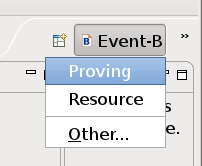
\includegraphics{img/tutorial/tut_08_switch_perspective.png}
	\caption{Switch Persepctive}
	\label{fig_tut_08_switch_perspective}
\end{center}
\end{figure}

\warning{If the Proving Perspective is not available in the menu, select \textsf{Other... $\rangle$ Proving}. This will open a new window which shows all available perspectives.}

We should now see the window in Figure \ref{fig_tut_08_proving_perspective}. 

\begin{figure}[!ht]
\begin{center}
	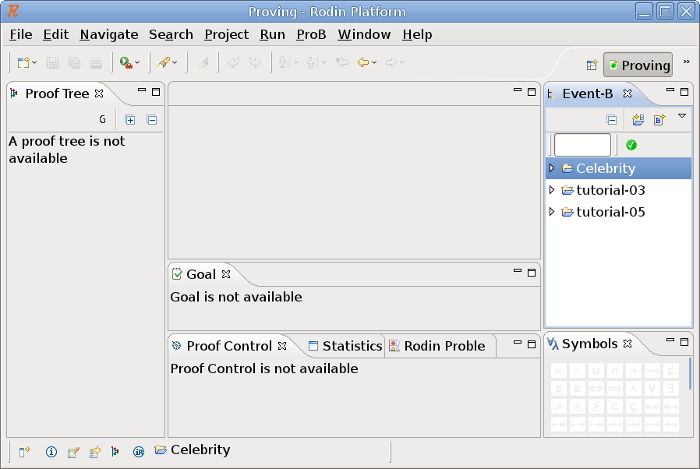
\includegraphics{img/tutorial/tut_08_proving_perspective.png}
	\caption{Rodin Proving Perspective}
	\label{fig_tut_08_proving_perspective}
\end{center}
\end{figure}

The \texttt{Proving Perspective} contains three new important views:

\begin{description}
	\item[Proof Tree View (\ref{proof_tree_view})] Here we see a tree of the proof that we have done so far and the current position in it. By clicking in the tree, we can navigate inside the proof. Currently, we have not started with the proof, so there is no new place to move to.
	\item[Proof Control View (\ref{proof_control_view})] This is where we perform interactive proofs.
	\item[Goal View (\ref{goal_view})] This window shows what needs to be proved at the current position inside the proof tree.
\end{description}

Expand the \texttt{Celebrity\_1} machine in the \textsf{Event-B Explorer}. Then expand the \textsf{Proof Obligations} section. We can see that the auto prover (\ref{auto_prover}) did quite a good job. Only three proofs have not been completed\footnote{Interestingly enough, this number can vary: Provers can be configured in the preferences, and changes there can have an impact on the ability to automatically discharge proofs.  In addition, all provers have time-outs.  On a slow machine, some proof obligations may not get discharged, compared to a faster machine with the same timeout.}  (a completed proof is indicated by a green check). 

%Except for the last one of them, all of them could be proved with a different external prover, but in order to learn a few new techniques, we will prove them with the so called ``p0 prover'' (\ref{p0_prover}). The p0 prover uses all selected hypotheses (the ones in Selected Hypotheses View).

Let's start with the proof \textsf{remove\_1/inv2/INV} of \texttt{Celebrity\_1}. To do this, double click on the proof obligation \textsf{remove\_1/inv2/INV}.

%\begin{figure}[!ht]
%\begin{center}
%	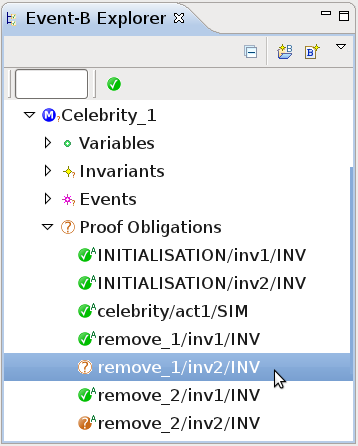
\includegraphics{img/tutorial/tut_08_proof1.png}
%	\caption{Rodin Proving Perspective}
%	\label{fig_tut_08_proving_perspective}
%\end{center}
%\end{figure}

We should now see the window as shown in Figure \ref{fig_tut_08_proof_obligation}.

\begin{figure}[!ht]
\begin{center}
	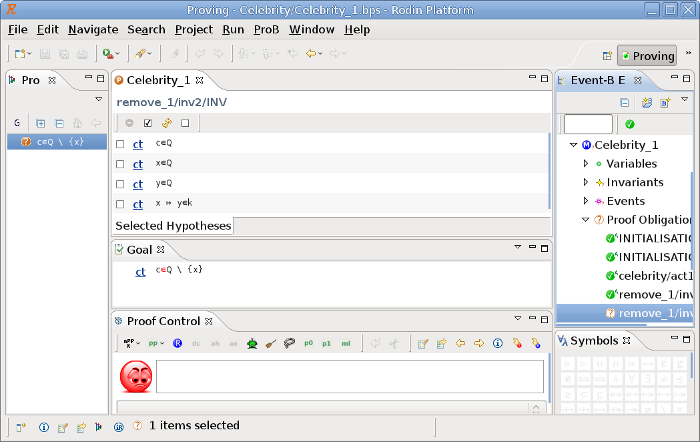
\includegraphics{img/tutorial/tut_08_proof2.png}
	\caption{Proof Obligation}
	\label{fig_tut_08_proof_obligation}
\end{center}
\end{figure}

\info{Make sure that you understand the different buttons in the \textsf{Proof Control View} (\ref{proof_control_view}).}

In order to prove the proof obligation, it suffices to prove \textsf{$x \neq c$}. Type this into the \textsf{Proof Control View} (\ref{proof_control_view}) and press the \textsf{\icon{rodin/ah_prover.png} button}. 

\info{In order to revert a step, click on a node in the \texttt{Proof Tree View} and click on the \icon{rodin/pn_prover.png} button in the \texttt{Proof Control View} or open the context menu of a node and select \texttt{Prune}.}

The new goal is $\lnot x = c$. Now, try selecting the right hypotheses by yourself in order to complete the proof. To do this, click on the \icon{rodin/sh_prover.png} button in the \textsf{Proof Control View}. On the left side we should see now the \textsf{Selected Hypotheses View} (see Figure \ref{fig_tut_08_search_hypothesis}). If you cannot find the right hypotheses, you may also just select all hypotheses. To add the selected hypothesis to the \textsf{Selected Hypotheses View} just click on the \icon{rodin/add.png} button. 

\begin{figure}[!ht]
\begin{center}
	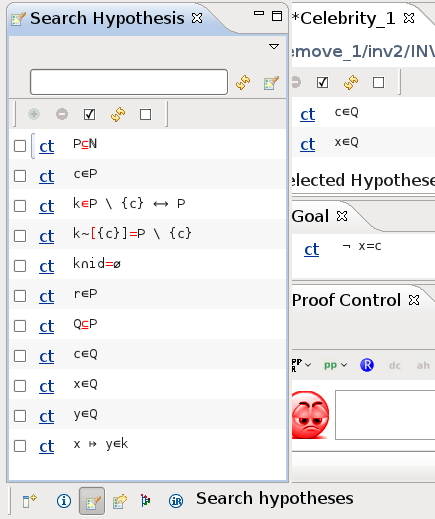
\includegraphics{img/tutorial/tut_08_search_hypothesis.png}
	\caption{Search Hypothesis View}
	\label{fig_tut_08_search_hypothesis}
\end{center}
\end{figure}

Now click on the \textsf{p0} button to prove the goal $\lnot x = c$ with the \textsf{Predicate prover on selected hypothesis}. The goal should be discharged and the \textsf{Proof Control View} should now show the original goal $c \in Q \setminus {x}$. Click a second time on the \textsf{p0} button in order to finalize the proof. The smiley in the \textsf{Proof Control View} should now become green indicating that all sequents of the proof tree are discharged as shown in Figure \ref{fig_tut_08_proof_final}.

\begin{figure}[!ht]
\begin{center}
	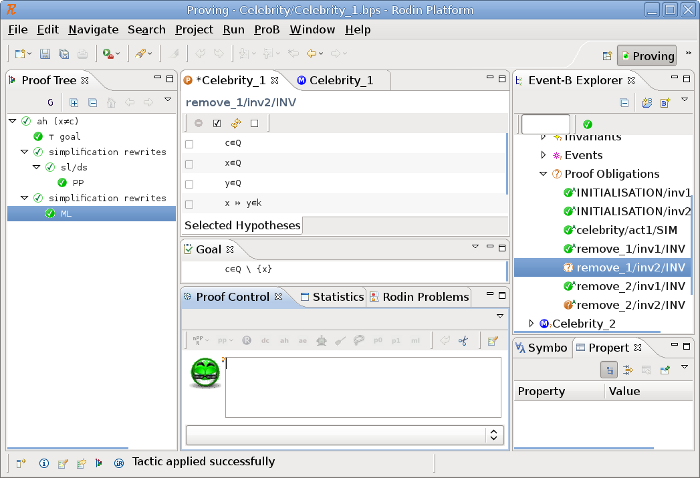
\includegraphics{img/tutorial/tut_08_proof_final.png}
	\caption{The green smiley indicates that all sequents of the proof tree are discharged}
	\label{fig_tut_08_proof_final}
\end{center}
\end{figure}

After saving the proof, the proof obligation \textsf{remove\_1/inv2/INV} in the \textsf{Event-B Explorer} should also become a green chop.

\info{There are alternative ways to prove the proof obligation. For instance, we can use the \icon{rodin/lasoo_prover.png} button to load those hidden hypotheses that contain identifiers in common with the goal into the \textsf{Selected Hypotheses View}, and we can also use it with the selected hypotheses.}

In order to move to the next undischarged proof obligation, you may also use the \textsf{Next Undischarged PO button} (\icon{rodin/next_prover.png}) of the \textsf{Proof Control View} (\ref{proof_control_view}). The next proof can be solved the same way as the last one.

\info{As an exercise, try to prove \texttt{Celebrity\_2}. A small hint: We have to fill in an existential quantifier. First, look in the list of hypothesis to see if you find any variable that is in P and select that hypothesis. Then instantiate \textsf{b'} and \textsf{R'} correctly (For instance, if you want to instantiate \textsf{b'} with \textsf{c}, then \textsf{$P \backslash \{ c\}$} is a good choice for \textsf{R'}) by typing the instantiations in the \textsf{Goal View} (\ref{goal_view}) and then clicking on the red existential quantifier. Now all open branches of the proof tree can be proved with \textsf{p0}. After this, we have completed all the proofs, and the model is ready for use. } 

\subsection{Prooving --- an Art or a Science?}

Prooving can be quite frustrating, both for beginners and advanced users.  Especially beginners sometimes get the impression that proofing is just ``clicking around'' that sometimes works and sometimes doesn't.  And when it works, it's not really clear why --- the proof tree is also difficult to read, even for experienced users.  We provided some additional guidance on proovers in Section~\ref{use_provers_effectively} that may be of help.

